\section{Problema 1}
\subsection{Enunciado}
Hay que encontrar la longitud de la meseta más grande de la unión ordenada de dos arreglos ordenados crecientemente (no estricto),
definiendo a la meseta como el subcojunto de números consecutivos iguales.

\subsection{Soluci\'on}
El problema presenta dos subproblemas a resolver: realizar la unión ordenada y encontrar la longitud de dicha meseta.
Para el primer subproblema, utilizaremos el algoritmo de Merge ya conocido por Merge-Sort en el que se irán recorriendo linealmente ambos arreglos, tomando en cuenta que están previamente ordenados y se irán colocando, en un nuevo arreglo de tamaño de la longitud 
de los arreglos de entrada, los valores de dichos arreglos de forma ordenada.
Una vez encontrada la unión ordenada, buscamos la longitud de la meseta más grande.
La idea consiste en recorrer linealmente el arreglo obtenido previamente e ir contando todos los valores iguales consecutivos encontrados. En el momento que el siguiente valor al evaluado sea distinto significa que es el inicio de otra meseta y hay que chequear si la longitud de la meseta anterior es la máxima hasta el momento. Para ello, utilizaremos una variable como acumulador que dentro del caso que el siguiente valor a evaluar sea distinto y el contador de la meseta actual sea mayor al anterior (en caso de existir), se acumulará esta nueva longitud en dicha variable.
Notese que, al final del algoritmo se devuelve acum + 1, esto es debido a que empezamos a contar a partir de una meseta mayor a dos,
anotando en contador solo 1, 
ya que al saber que la entrada es no vacía, se estaría guardando el valor de la longitud de las mesetas de longitud uno que eso siempre existe al ser no vacía.

\subsection{Pseudoc\'odigo}

\begin{codebox}
\Procname{$\proc{arrayLongMeseta}$ (\textbf{in} $array1$ ; \textbf{in} $array2$)}{res}{Int}
\li	ArrayMerged = MergeOrdenado(Array1,Array2)
\li     cont = 0;	
\li     acum = 0;
\li     Mientras( i $<$ $|$ArrayMerged$|$ - 1) \Do
\li          \textbf{si} (ArrayMerged[i] == ArrayMerged[i+1]) \Do
\li             cont ++; \RComment Si estoy dentro de la misma meseta, sigo contando
\End
\li 	     \textbf{sino}  \Do
\li 	     \textbf{si} (cont $>$ acum) \Do
\li		acum = cont; \RComment Si estoy fuera de la meseta y el contador previo supera mi acumulador, lo guardo
\End
\li 	     cont = 0; \RComment Como estoy fuera de la meseta, reseteo contador
\End
\End
\li 	     \textbf{si} (cont $>$ acum) \Do
\li		acum = cont; \RComment Esto es para el último caso
\End
\li	     devuelvo acum + 1;

\end{codebox}


\subsection{Analisís de complejidad}

\begin{codebox}
\li	ArrayMerged = MergeOrdenado(Array1,Array2) \\
Este algoritmo lo tomaremos como conocido junto a su complejidad O($|$Array1$|$ + $|$Array2$|$)\\
\\

Al no tener llamadas recursivas, el análisis del algoritmo es bastante simple e intuitivo.

\li     Mientras( i $<$ $|$ArrayMerged$|$ - 1) \Do \\
Se recorren todos los elementos del ArrayMerged sin excepción
\li          \textbf{si} (ArrayMerged[i] == ArrayMerged[i+1]) \Do \RComment O(1)
\li             cont ++; \RComment O(1)
\End
\li 	     \textbf{sino}  \Do \RComment O(1)
\li 	     \textbf{si} (cont $>$ acum) \Do \RComment O(1)
\li		acum = cont; \RComment \RComment O(1)
\End
\li 	     cont = 0; \RComment O(1)
\End
\End
\li 	     \textbf{si} (cont $>$ acum) \Do \RComment O(1)
\li		acum = cont; \RComment O(1)
\End
\li	     devuelvo acum + 1;
\\
Entonces es $\sum\limits_{i=0}^n O(1)$, donde n es $|$Array1$|$ + $|$Array2$|$ \\
\\
Entonces la complejidad es: O(2*($|$Array1$|$ + $|$Array2$|$))\\
\\
Lo que implica: O($|$Array1$|$ + $|$Array2$|$)\\

\end{codebox}





\subsection{Tests y Gráficos}
En el test del problema en cuestión, consideramos que no hay peores ni mejores casos posibles.
Por ende, cualquier caso elegido para testear nos representa lo mismo.
Por ende, probamos unos casos random para ver la linealidad en base a la longitud de la unión de los arreglos.
Para probar hicimos script como test que genera arreglos ordenados aleatorios (tanto a longitud como los valores internos).
El test en si, toma estos valores y escribe la cantidad de ciclos obtenidos para cada longitud retornando esos valores en un archivo.
El siguiente gráfico está basado en ese resultado.


\begin {center}
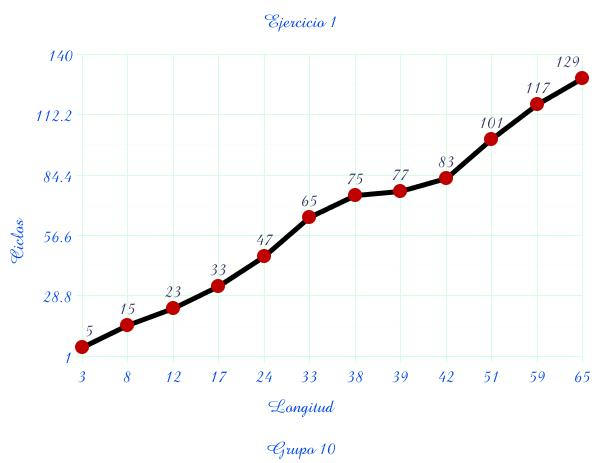
\includegraphics[width=12cm]{./graphEj1.jpg}
% grafico.eps: 0x0 pixel, 300dpi, 0.00x0.00 cm, bb=50 50 410 302
\end {center}

Como se puede observar, tomando la cantidad de ciclos utilizados en base a la longitud se nota claramente la linealidad
del algoritmo.


\subsection{Conclusiones}
Como pudimos ver en el análisis de complejidad nuestro algoritmo cumple con la complejidad requerida y esta complejidad es igual para cualquier dato de entrada, es decir, que no hay $"$casos límite$"$, la complejidad es de O($|$x$|$+$|$y$|$) siempre.
Destacamos en este ejercicio la practicidad de generar tests ya que si en algún momento se decide hacer un cambio, y para un primer intento de demostración de correctitud,
correr los tests y ver los gráficos de los mismos, es un buen parámetro para empezar. Esto es debido a que los inputs de los test se generan automáticamente (de forma
aleatoria y la cantidad de inputs deseados) y luego sobre cada uno de esos datos de entrada se corre el algoritmo que termina escribiendo el resultado de cada ejecución en
el arhcivo .out.
